\documentclass{article}
\usepackage{xeCJK}
\usepackage{amsmath}
\usepackage{graphicx}
\usepackage{svg}


\setCJKmainfont{Microsoft YaHei}
\linespread{1.5}
\setlength{\parindent}{0pt}

\begin{document}
1. \\
(1) $2^{A} = \{\emptyset, \{\varepsilon\}, \{0\}, \{00\}, \{\varepsilon, 0\}, \{\varepsilon, 00\},\{0, 00\}, \{\varepsilon, 0, 00\}\}$ \\
(2) $A \times B = \{\{\varepsilon, 0\}, \{\varepsilon, 1\}, \{0, 0\}, \{0, 1\}, \{00, 0\}, \{00, 1\}\}$ \\
2.\\
\begin{figure}[htbp]
	\centering
    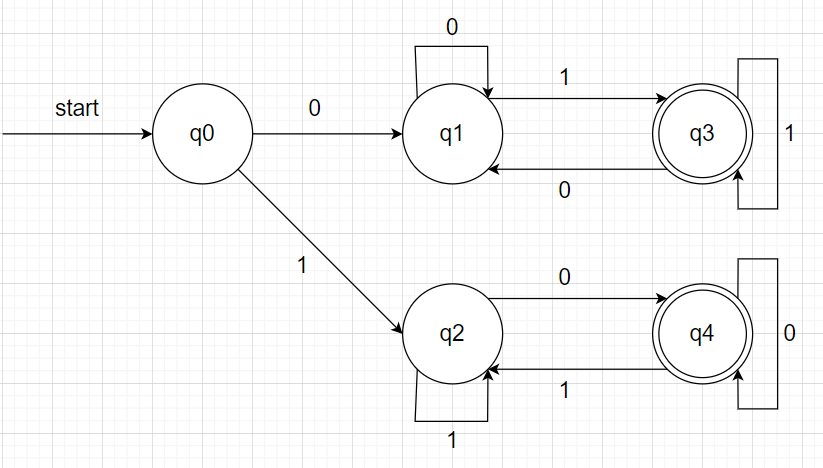
\includegraphics[width=1\columnwidth,height=!]{DFA1.png}
	\caption{DFA1}
\end{figure}
\\
3.\\
\begin{figure}[htbp]
	\centering
    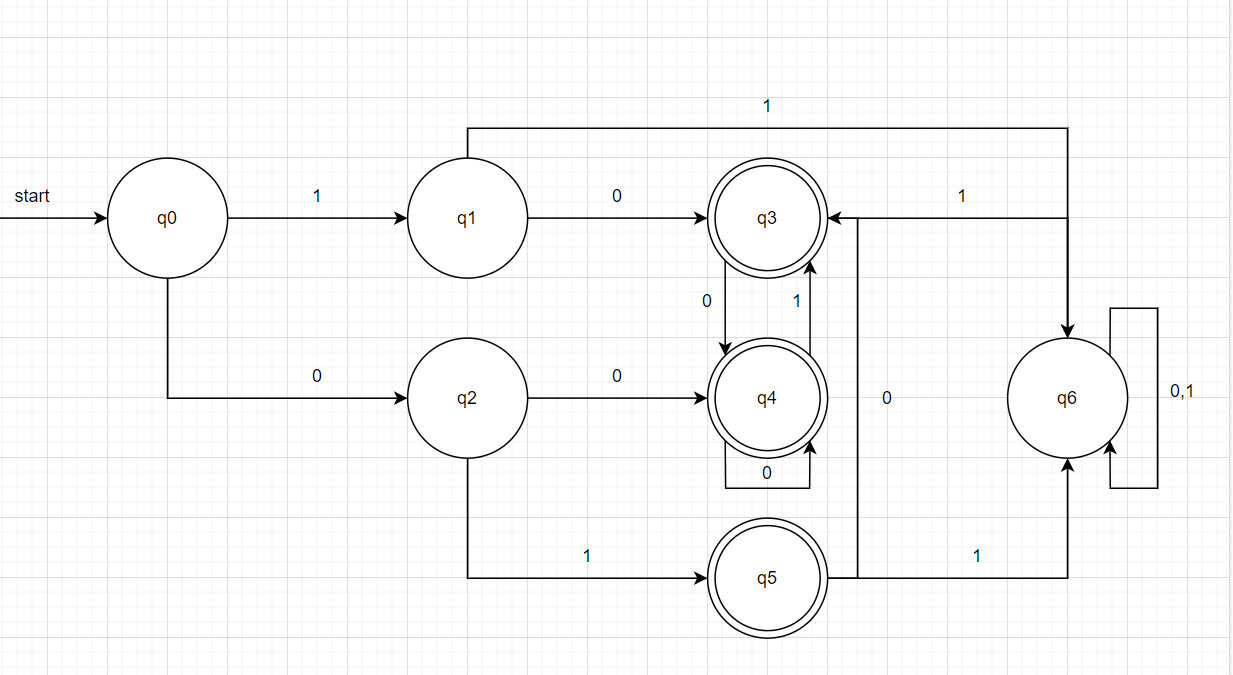
\includegraphics[width=1\columnwidth,height=!]{DFA2.png}
	\caption{DFA2}
\end{figure}

\end{document}